\documentclass[11pt,a4paper]{article}
\usepackage[margin=2.2cm]{geometry}
\usepackage{graphicx,booktabs,url,amsmath}
\usepackage[hidelinks]{hyperref}
\graphicspath{{../../fullsim_analysis/results/bench/2026-10-22/}{../../fullsim_analysis/results/bench/2026-10-21/}}
\title{Bench data of 22 October 2026: menu 1 with five boards}
\author{CaLibrated AUtomatic DocumEnt (CLAUDE), supervised by J. J. G\'omez-Cadenas}
\date{23 October 2026}
\begin{document}
\maketitle

Data measured by Laura Navarro on 22 October 2026 with five A5202 boards and the PET CAEN DAQ,
copied from \path{hyperion:/data/lnavarro/26_10_caen_measurements_jj}. The runs repeat bench
note 1 (Citiroc noise) after JMB solved the saturation of 21 October. Boards are numbered as in
the DAQ (board 0--4 = chain,node 0,0 / 0,1 / 1,0 / 1,1 / 1,2), channels 0--63; the two Citirocs
of a board are channels 0--31 and 32--63. The problems found so far, and their status, are
kept in a findings log (F1--F10), cited below.

\section{Data received}

\begin{center}
\small
\begin{tabular}{llll}
\toprule
Runs & Step of note 1 & HG shaping & HoldDelay \\
\midrule
26, 27, 28 & 1: noise against shaping & 25, 50, 87.5 ns & 0 ns \\
29--33 & 2: pedestal against HoldDelay & 25 ns & 96, 200, 296, 400, 496 ns \\
34 & 3: stability & 25 ns & 0 ns \\
\bottomrule
\end{tabular}
\end{center}

\noindent Each run has 10\,012--10\,016 periodic triggers (1~ms) read by the five boards, with
no trigger lost. The low gain is at 87.5~ns in all runs. \texttt{HV\_Vbias} = 40.7~V with
\texttt{HV\_IndivAdj} = 0, so the SiPMs see 36.5~V, below breakdown (F2); the HV current is
0.2--0.35~$\mu$A. The detector temperature is 24.0--25.0~$^\circ$C on all boards. The logbook
has one row per run and board and agrees with the files. The DAQ now records
\texttt{PeakDetectorMode} (PEAK\_STRETCH, applied on all boards), which shows that it includes
the pull requests merged on 20 October.

\section{What works}

\begin{itemize}
\item \textbf{The saturation is gone} (F1). No value of any channel is at 8191.
\item \textbf{Pedestals.} The mean of the high gain is different in each channel, between 50
  and 310 ADC counts (Figure~\ref{fig:ped}), and the low gain between 55 and 280. Between
  run 26 and run 34, taken 23 minutes apart with the same settings, the pedestals move by
  $-0.4$ counts on average and by at most 1.6 counts: they are stable.
\end{itemize}

\begin{figure}[h]
\centering
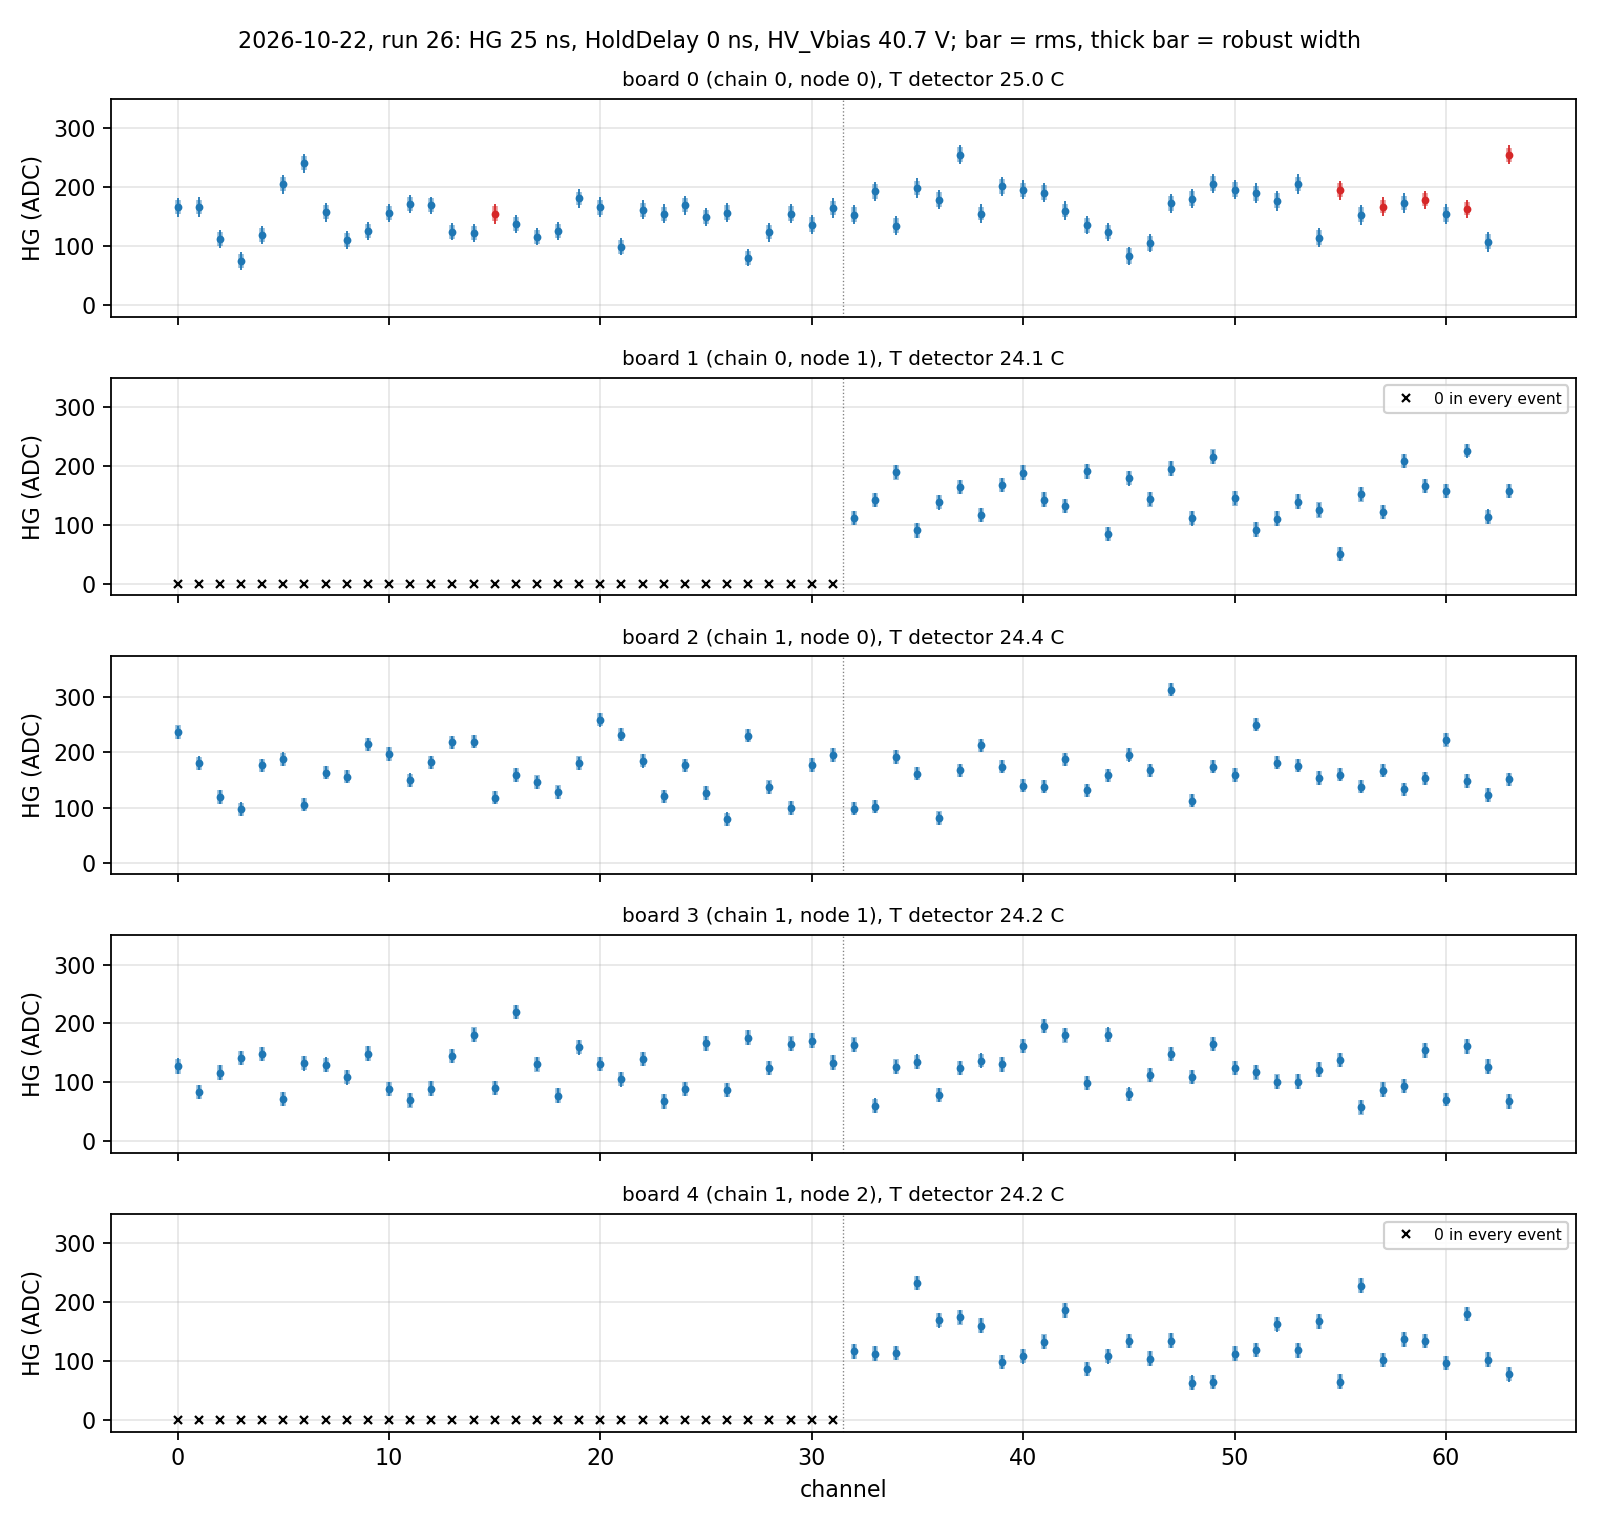
\includegraphics[width=0.92\textwidth]{bench_pedestals.png}
\caption{Run 26 (HG 25~ns, HoldDelay 0): mean of the high gain against the channel for each
board, with the rms as error bar and the robust width (interquartile range / 1.349) as a
thicker bar. Crosses at zero: channels that read 0 in every event. In red, the channels of
board 0 without avalanches in the staircases of 21 October (F4).}
\label{fig:ped}
\end{figure}

\section{Noise}

The rms of the high gain is 12--13 ADC counts at the three shapings, and that of the low gain
about 6 counts, the same on all boards. Because the 32 channels of a chip are read at the same
trigger, the noise can be split into a \textbf{coherent} part, the event-by-event shift shared
by the whole chip (the mean of the deviations of its 32 channels), and an \textbf{incoherent}
part, that of each channel after subtracting this shift. Figure~\ref{fig:shaping} shows both
against the shaping time.

\begin{itemize}
\item \textbf{The noise barely depends on the shaping.} The simulation assumes white series
  noise, which would be 1.87 times larger at 25~ns than at 87.5~ns. The total noise is instead
  0.94 times as large; the incoherent part grows only by 1.13, and the coherent part falls
  (0.72).
\item \textbf{A quarter to 40\% of the variance is coherent} (5.9 counts at 25~ns, 8.2 at
  87.5~ns). The coherent noise belongs to the board: it is correlated by 0.6--0.8 between the
  two chips of a board and not at all between boards. In the sum of the 64 channels, which
  gives the energy, it adds linearly and dominates: about 380 counts against 85 from the
  incoherent part at 25~ns.
\item \textbf{The pedestal rises slowly with the window.} With a longer HoldDelay the pedestal
  rises and narrows, as expected for the peak stretch, but at 296~ns it has risen by 0.5--0.6
  rms where the model predicts 2.2, and it is still rising at 496~ns.
\item \textbf{The low gain} has 0.45 times the noise of the high gain at the same shaping,
  where the model assumes the same noise in counts.
\end{itemize}

\noindent These results, the hypotheses that could explain them (a low-frequency noise, the
bias line of the SiPMs, a non-ideal peak detector) and the measurements that would test them
are discussed in the note \emph{Noise of the Citiroc front end: model and bench data}.

\begin{figure}[h]
\centering
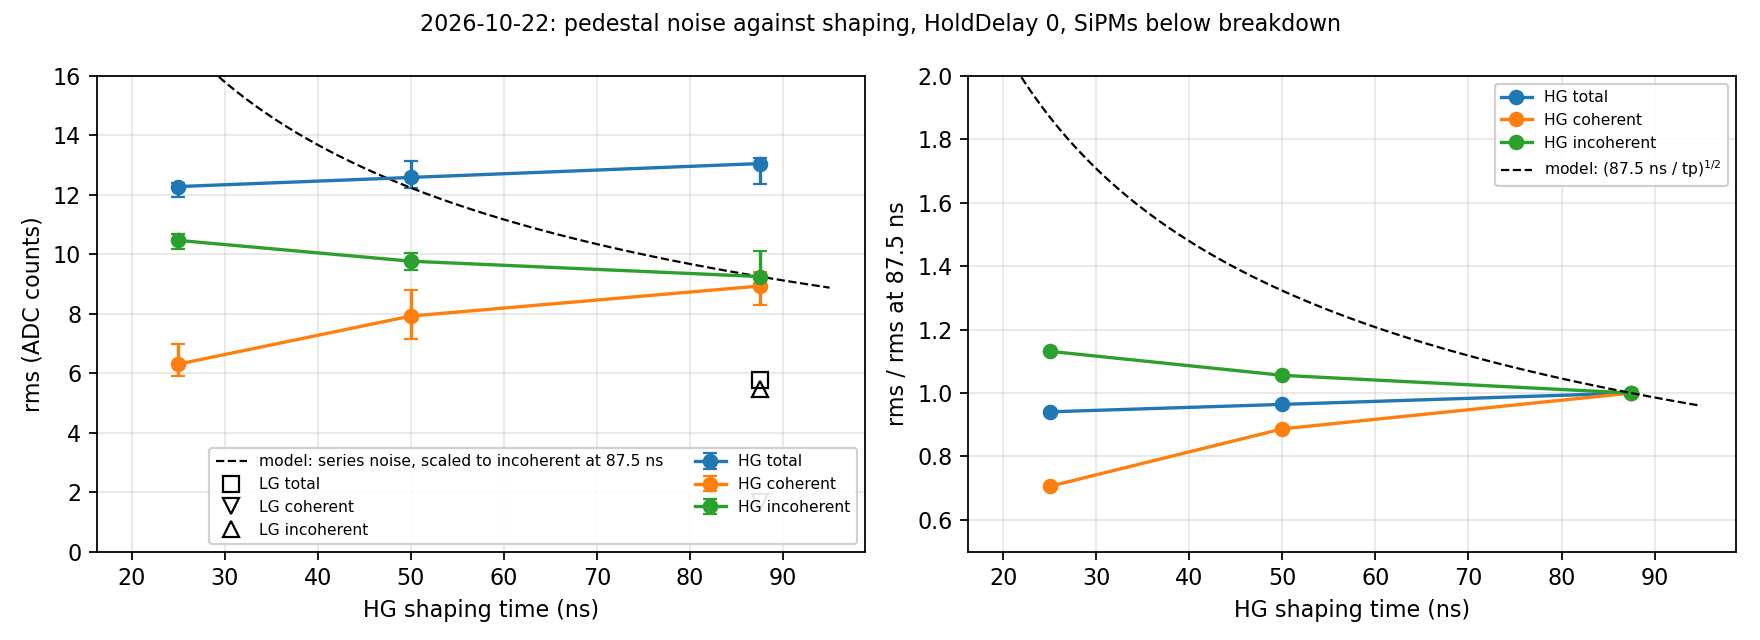
\includegraphics[width=\textwidth]{noise_vs_shaping.png}
\caption{Runs 26--28: total, coherent and incoherent noise of the high gain against the
shaping time (median over the eight chips read, bars from the lowest to the highest chip),
and the low gain at 87.5~ns. Left, in ADC counts, with the model scaled to the incoherent
noise at 87.5~ns; right, divided by the value at 87.5~ns.}
\label{fig:shaping}
\end{figure}

\section{Problems}

\begin{itemize}
\item \textbf{Half of boards 1 and 4 reads zero (F7).} Channels 0--31 of boards 1 and 4 give 0
  in every event, in both gains and all nine runs; channels 32--63 of the same boards are
  normal. The configuration stored in the files is the same for these two chips as for the
  others: readout, discriminators and preamplifiers enabled, the same gains, thresholds and
  shaping, and per-channel pedestal calibrations of 102--271 counts like those of the chips
  that work. \texttt{Pedestal} = 0 is not the cause either, since the live channels have
  essentially no value at zero. The same chip failing on two boards with a normal
  configuration points to the readout, presumably firmware or DAQ. 64 of the 320 channels
  have therefore no data. \textbf{JMB}: needs a fix in the readout; reading board 1 with
  Janus, CAEN's software, would tell whether the problem is in the DAQ.
\item \textbf{Common-mode jumps of board 0 (F10).} In 0.1--0.4\% of the events of runs 26--32,
  all the channels of board 0, on both chips, move together by 60--230 counts, up or down,
  often in two consecutive triggers (1~ms apart). This is what made board 0 look noisier in
  run 26: its rms is 15.9 counts, but its robust width is 11.9, the same as on the other
  boards. Runs 33 and 34 have no such events, and the other boards have none (board 3, one
  event in three runs). A shift of the whole board points either to its reference, supply or
  ground, or to the readout. \textbf{JMB}: is it hardware (power, ground, cabling of board 0)
  or firmware?
\item \textbf{Firmware (F9).} Board 2 runs firmware 0xa7070800, the others 0xa1230708. No
  effect is visible in the data: board 2 reads normally. \textbf{JMB}: is the difference
  intended, and could the firmware be behind F7 or F10?
\end{itemize}

\section{Channels without avalanches}

The staircases taken on 21 October on board 0, with the SiPMs above breakdown, scan the
threshold of the timing discriminator of each channel and count its rate
(Figure~\ref{fig:stair}). Above the noise plateau, which ends at 180--185 DAC in all
channels, the rate falls slowly with the steps of the dark-count spectrum (1, 2, 3 \ldots\ pe)
in 54 channels. Six channels, \textbf{15, 55, 57, 59, 61 and 63}, fall from the plateau to zero
within 10 DAC and count 0--4~Hz 30 DAC above the edge, against a median of $6\times10^5$~Hz:
they see no avalanches (F4). Since the SiPMs are connected, the signal is lost between SiPM and
Citiroc, in a bad contact or in the connector. Four more, \textbf{0, 2, 8 and 10}, count 7--10
times less than the median (F5).

\begin{figure}[h]
\centering
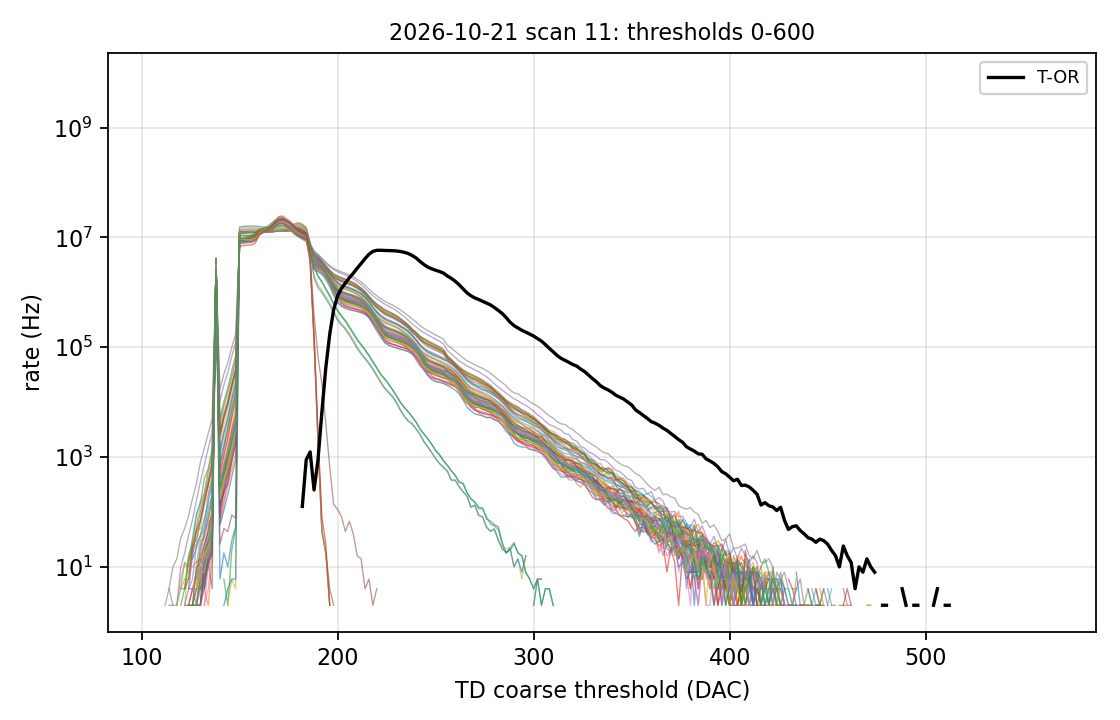
\includegraphics[width=0.6\textwidth]{staircase_11.png}
\caption{Staircase of 21 October (scan 11, board 0): rate of the timing discriminator against
its coarse threshold, one curve per channel, with the T-OR in black.}
\label{fig:stair}
\end{figure}

A SiPM at the input raises the noise of its preamplifier, so a channel with a bad contact
should also be quieter in the pedestal runs, which would allow the other boards to be checked
without staircases. Figure~\ref{fig:noise} shows the rms of each channel divided by the median
of its board: at 87.5~ns the six silent channels of board 0 sit at 0.82--0.87, but channels
with avalanches reach 0.81--0.89. The pedestal does not separate them, and the staircases of
all five boards are needed.

\begin{figure}[h]
\centering
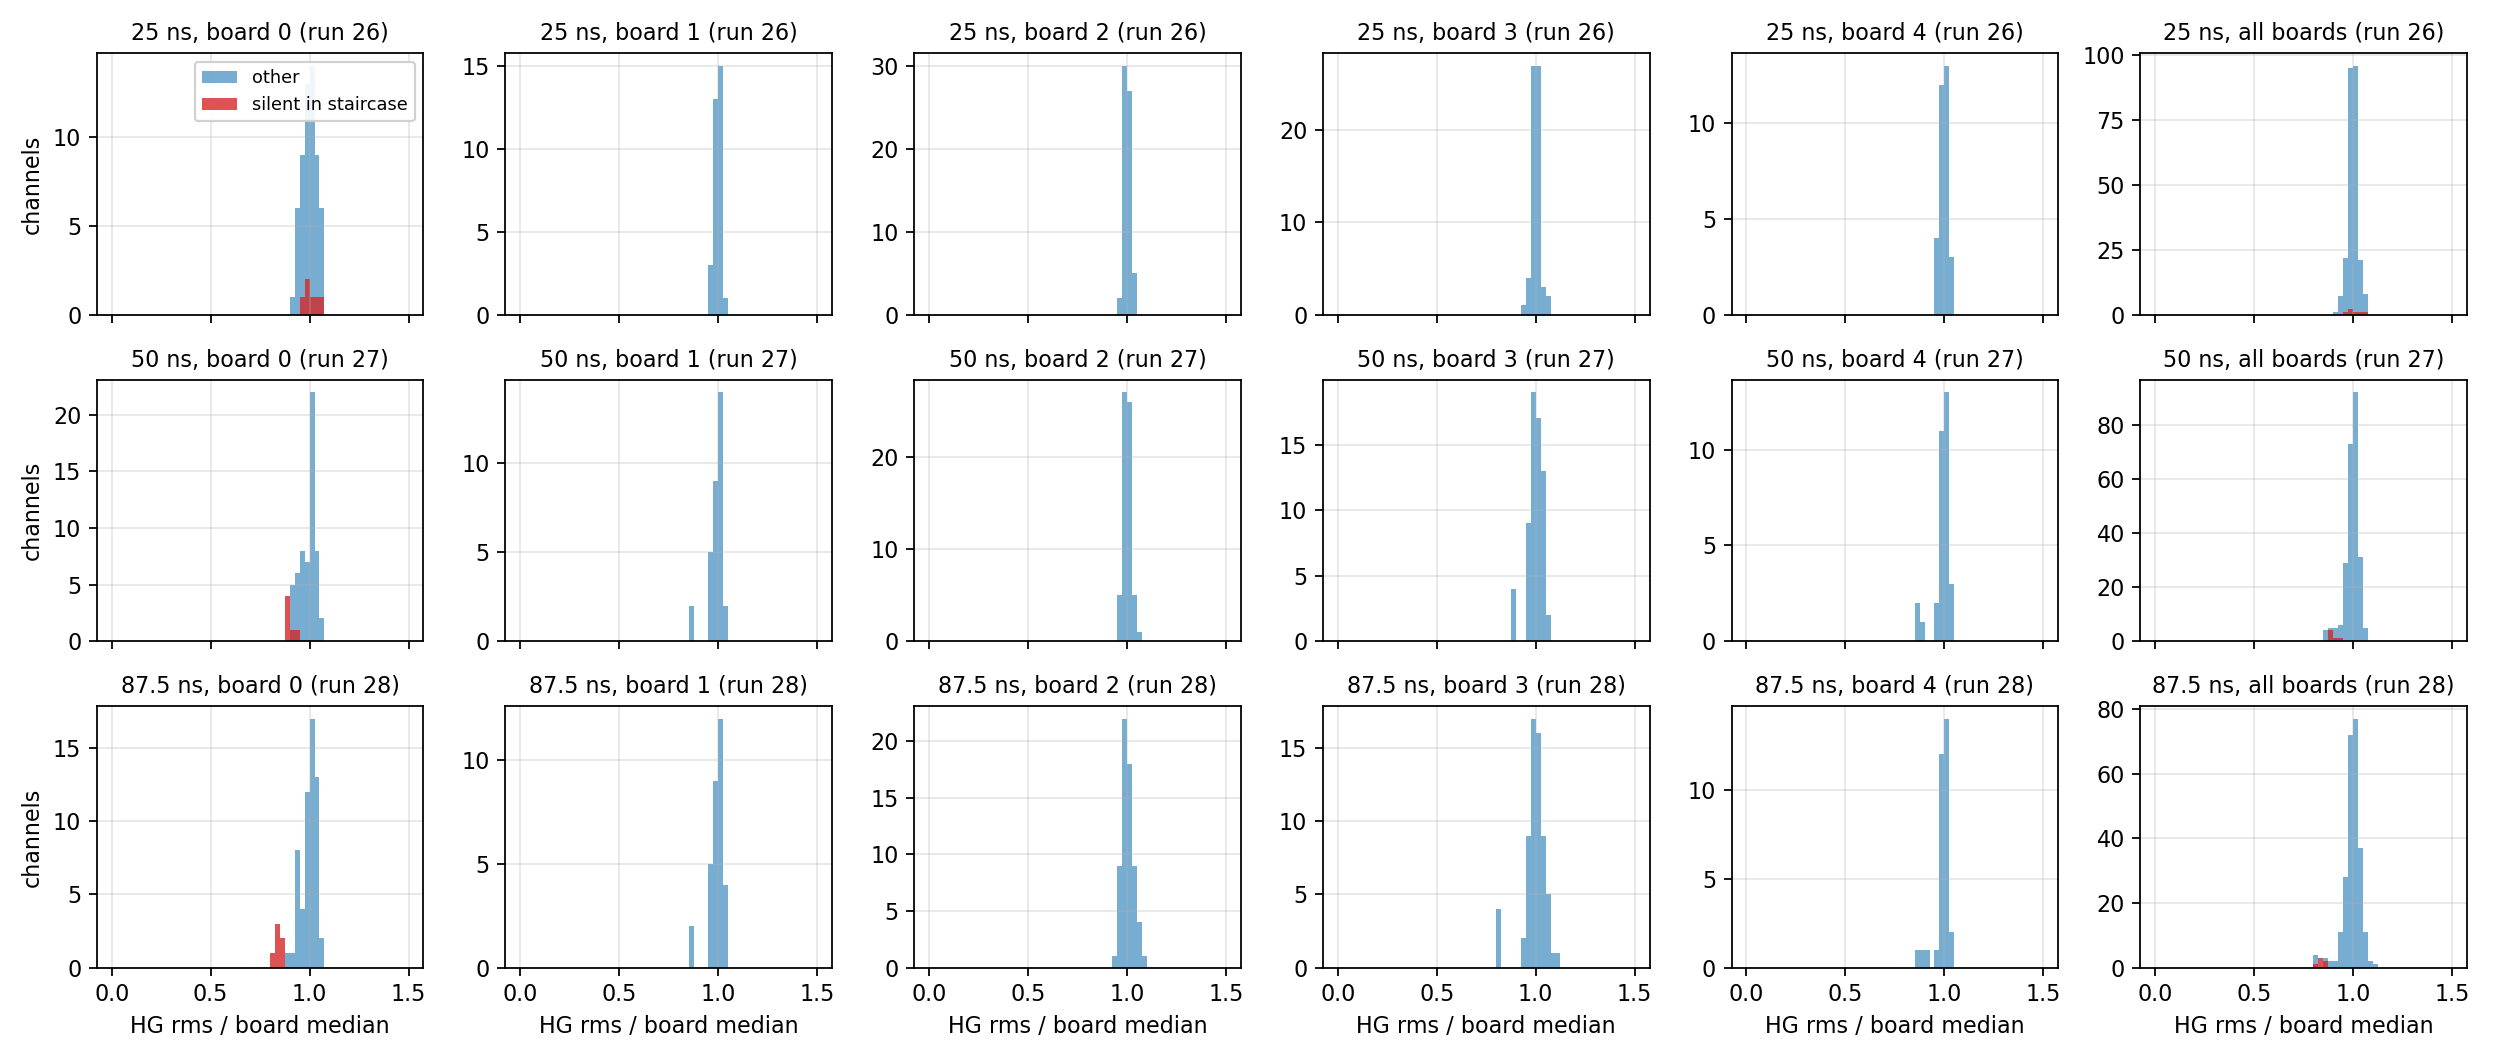
\includegraphics[width=\textwidth]{bench_noise.png}
\caption{Runs 26--28: rms of the high gain divided by the median of its board, one row per
shaping, one column per board and all boards together. In red, the six channels of board 0
silent in the staircases of 21 October.}
\label{fig:noise}
\end{figure}

\section{Two pedestal peaks in the plots grouped by node}

In the quick-look plots of these runs made at the bench, most channels of ``board 0'' and half
of the channels of ``board 1'' show two pedestal peaks, half of ``board 2'' shows nothing, and
only three boards appear. The plots group the measurements by the node number alone. The five
boards sit on two chains, boards 0 and 1 on chain 0 (nodes 0 and 1) and boards 2, 3 and 4 on
chain 1 (nodes 0, 1 and 2), so that grouping by node gives three groups and mixes boards:

\begin{itemize}
\item \textbf{Node 0} is boards 0 and 2. Each channel shows the pedestals of two different
  boards, hence two peaks, or one when the two pedestals happen to coincide.
\item \textbf{Node 1} is boards 1 and 3. In channels 0--31 board 1 reads 0 (F7) and a cut
  above 20 counts removes it, leaving board 3 alone; in channels 32--63 both boards are
  present and there are two peaks.
\item \textbf{Node 2} is board 4 alone, whose channels 0--31 read 0 (F7).
\end{itemize}

\noindent The positions of the two peaks agree channel by channel with the pedestals of the two
boards measured separately (run 26):

\begin{center}
\small
\begin{tabular}{lccl}
\toprule
Channel & Board 0 & Board 2 & Plot grouped by node 0 \\
\midrule
0 & 166 & 235 & peaks at about 165 and 235 \\
6 & 240 & 105 & peaks at about 100 and 240 \\
27 & 80 & 230 & peaks at about 80 and 240 \\
47 & 172 & 312 & peaks at about 170 and 310 \\
1, 57, 61 & 166, 167, 163 & 180, 166, 147 & one peak \\
\bottomrule
\end{tabular}
\end{center}

\noindent Figure~\ref{fig:mix} shows it directly: each board alone has one peak per channel, and
their sum reproduces the two peaks. The spectra of all channels of the five boards, each board
on its own, are in the appendix: one pedestal per channel, everywhere. There are no short
circuits to explain in these data, and no board is missing: the five are in the files.

\begin{figure}[h]
\centering
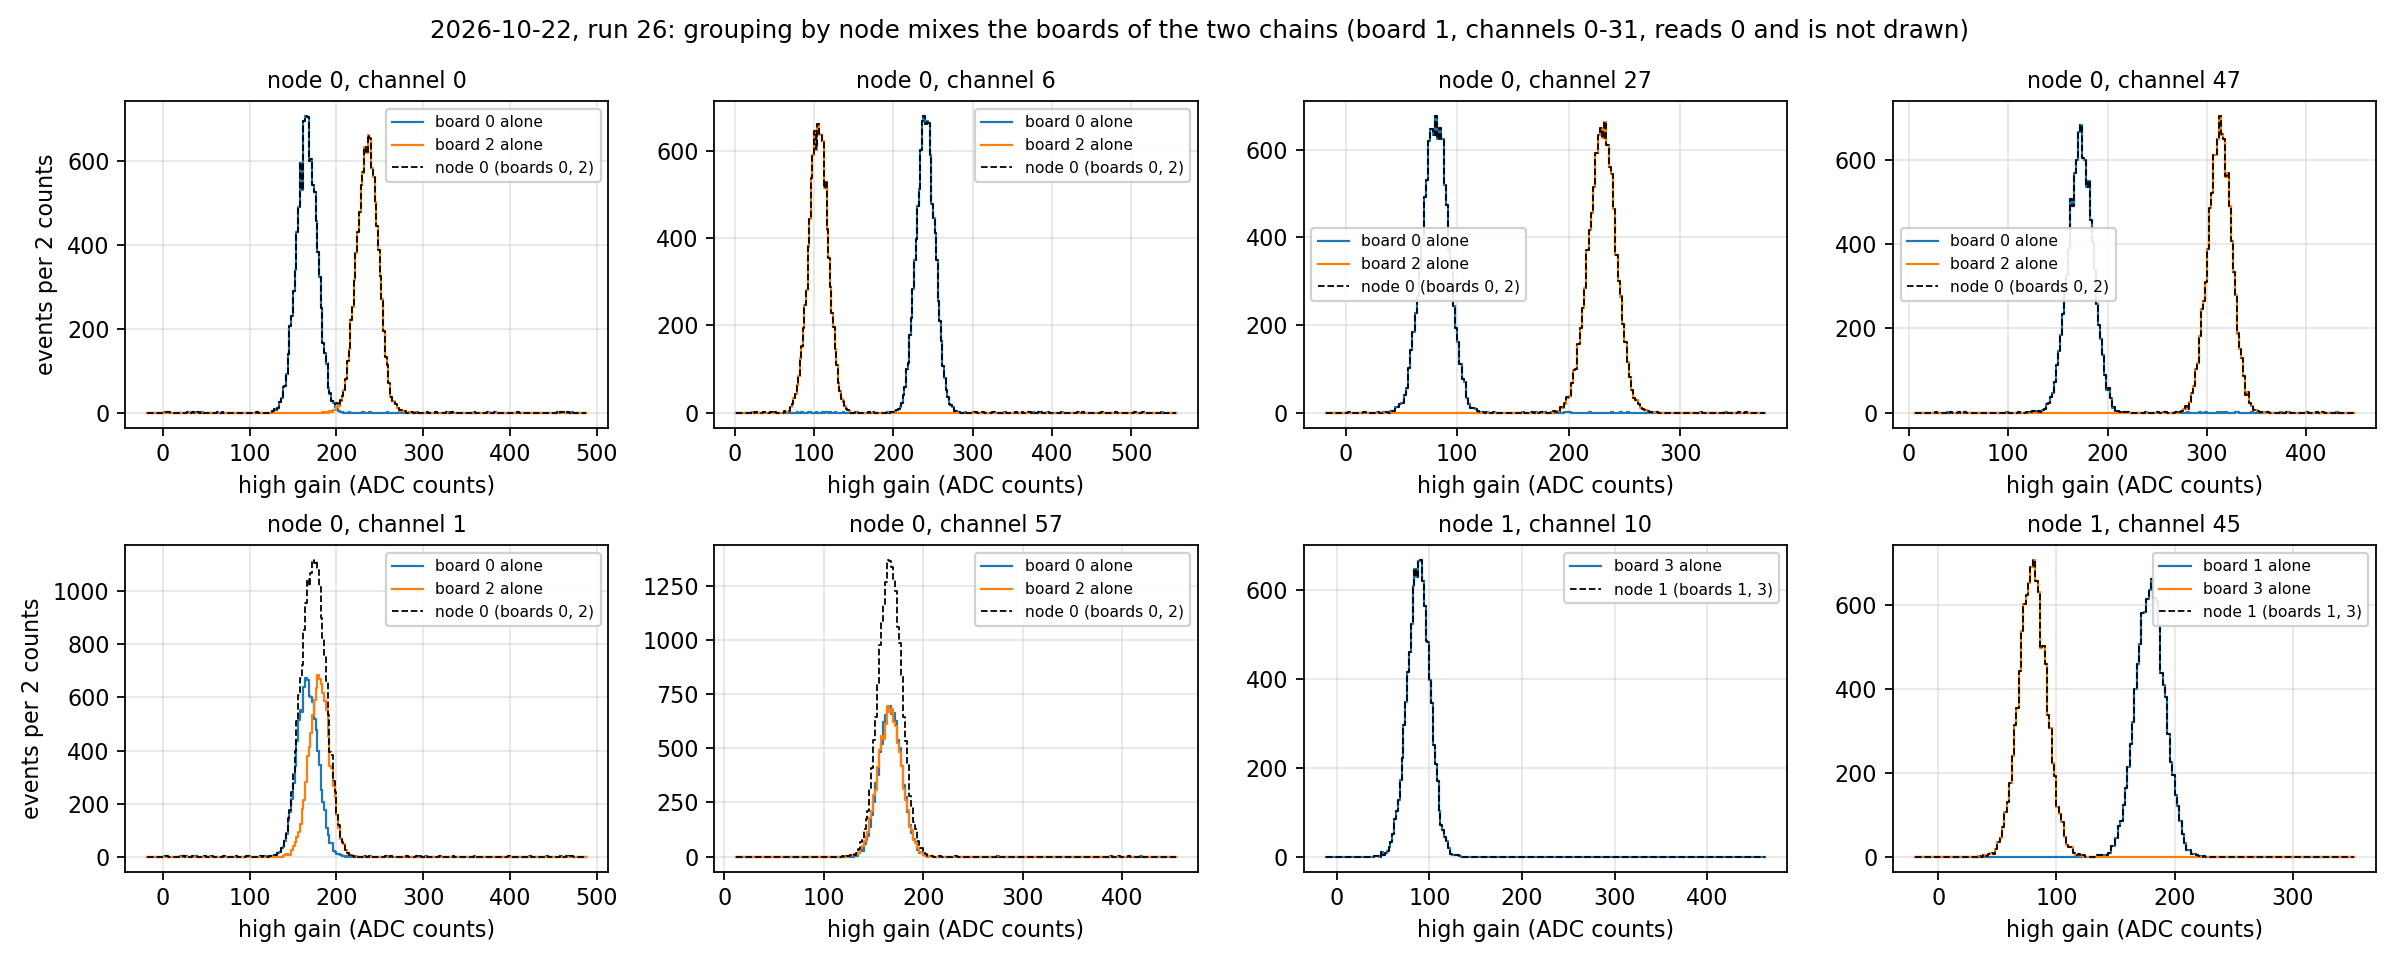
\includegraphics[width=\textwidth]{node_mixing.png}
\caption{Run 26, high gain: spectra of some channels for each board alone (solid) and for the
boards that share a node number added together (dashed), which is what a plot grouped by node
shows.}
\label{fig:mix}
\end{figure}

\paragraph{Recipe.} A board is identified by the pair (chain, node) of each measurement, never
by the node alone. Every run stores the table that numbers the boards, in
\path{manifest.json} (\path{execution_identity.topology.boards}) and in the event file
(\path{configuration/effective/boards}), with the fields board, chain and node. In a script:
\begin{verbatim}
boards = {(b["chain"], b["node"]): b["board"]
          for b in manifest["execution_identity"]["topology"]["boards"]}
board  = [boards[(c, n)] for c, n in zip(obs["chain"], obs["node"])]
\end{verbatim}
and the spectra are then made per board and channel. \textbf{Laura}: with this change the
plots of the five boards should look like those of the appendix.

\section{Requests}

\textbf{JMB}: the dead chips of boards 1 and 4 (F7), the common-mode jumps of board 0 (F10)
and the firmware of board 2 (F9), as above.

\medskip
\noindent\textbf{Laura}: menu 1 is complete, except for the 64 channels of F7, which will
need runs 26--34 repeated once JMB has solved it. The next session is menu 2 (bench note 2,
hold-delay scan), as written, with three corrections:
\begin{enumerate}
\item \texttt{HV\_Vbias} = 47.2~V. The note asks for about 43~V, but the board subtracts 4.2~V
  (F2), and 5~V of overvoltage needs about 43~V at the SiPM.
\item \texttt{FastShaperInput} = HG-PA, set explicitly. The DAQ now applies it, and the
  production configuration asks for LG-PA; the precaution of the note (staircase first, so
  that the fast shaper is left on the high gain) is no longer needed.
\item With five boards, the scan triggers on one channel of board 0 and the trigger masks of
  the other boards are set to zero. The staircase of step 1 is taken on all five boards: it
  will show which channels see their SiPM (F4, F5).
\end{enumerate}

\clearpage
\appendix
\section{Pedestal spectra of the five boards}

Spectra of the high gain of every channel, board by board (boards identified by chain and
node), in runs 26, 27 and 28 (HG shaping 25, 50 and 87.5~ns, HoldDelay 0).

\begin{figure}[p]
\centering
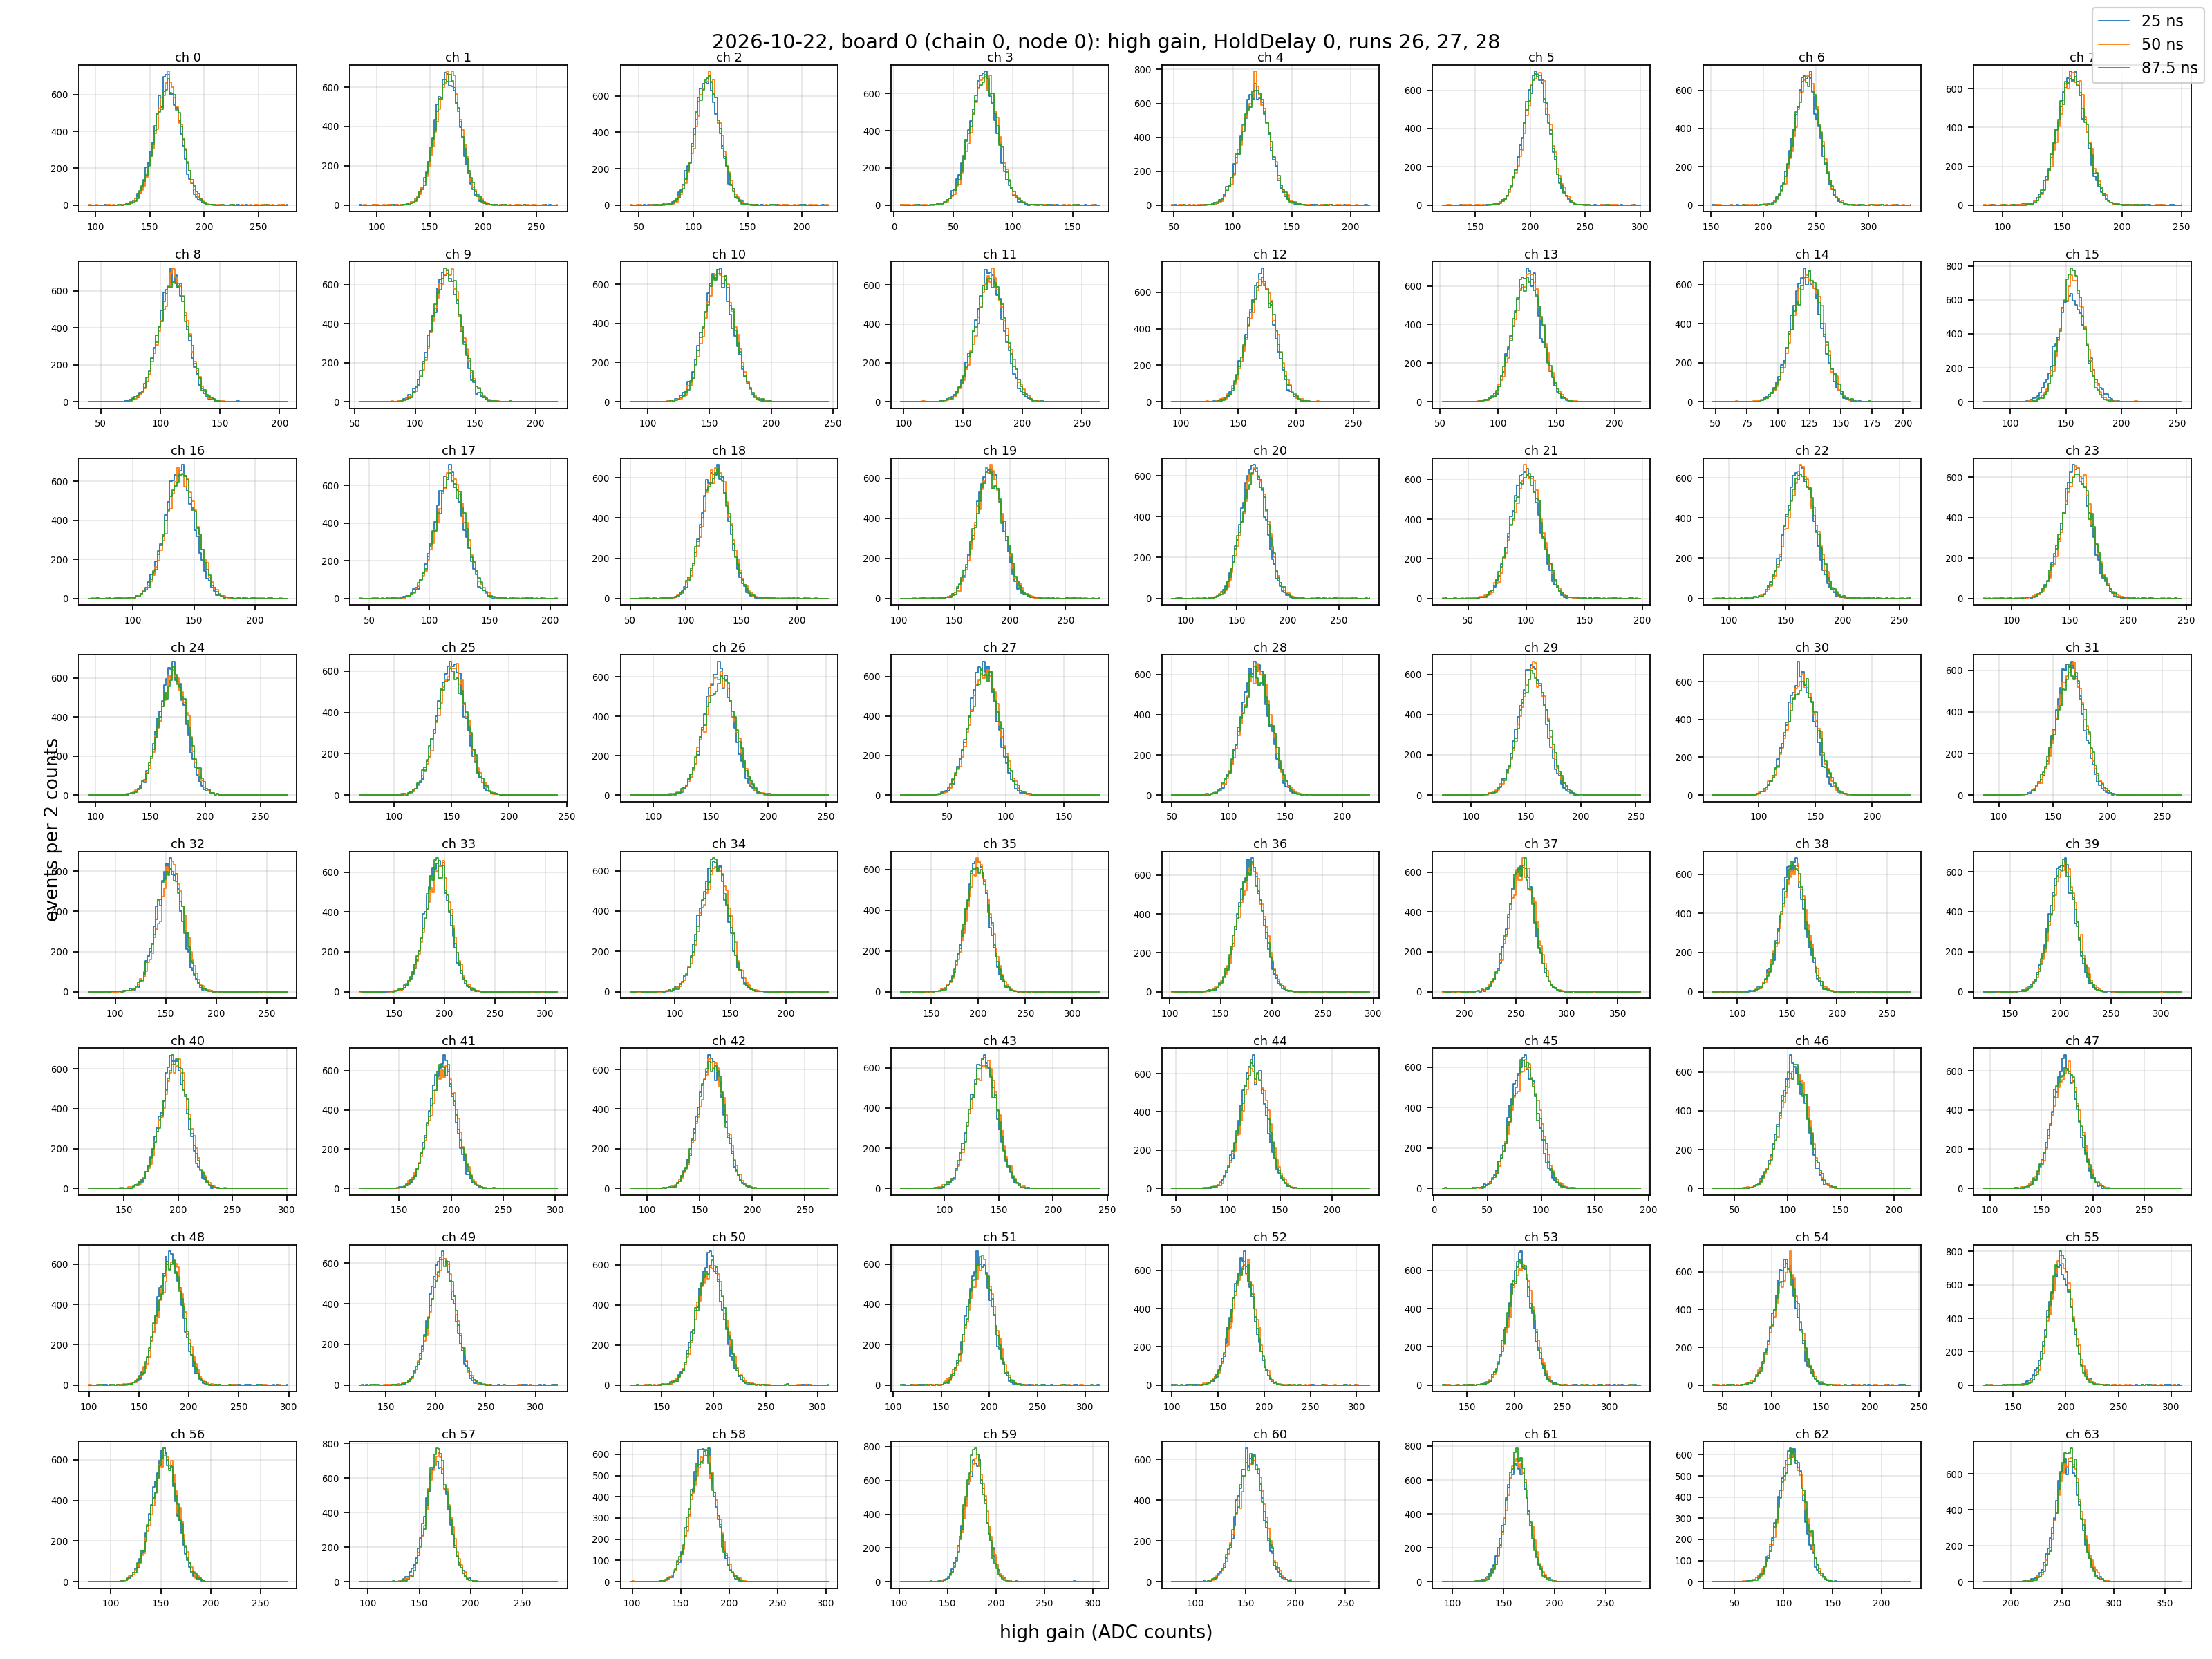
\includegraphics[width=\textwidth]{pedestal_spectra_board0.png}
\caption{Board 0: spectrum of the high gain of each channel in runs 26--28.}
\end{figure}
\begin{figure}[p]
\centering
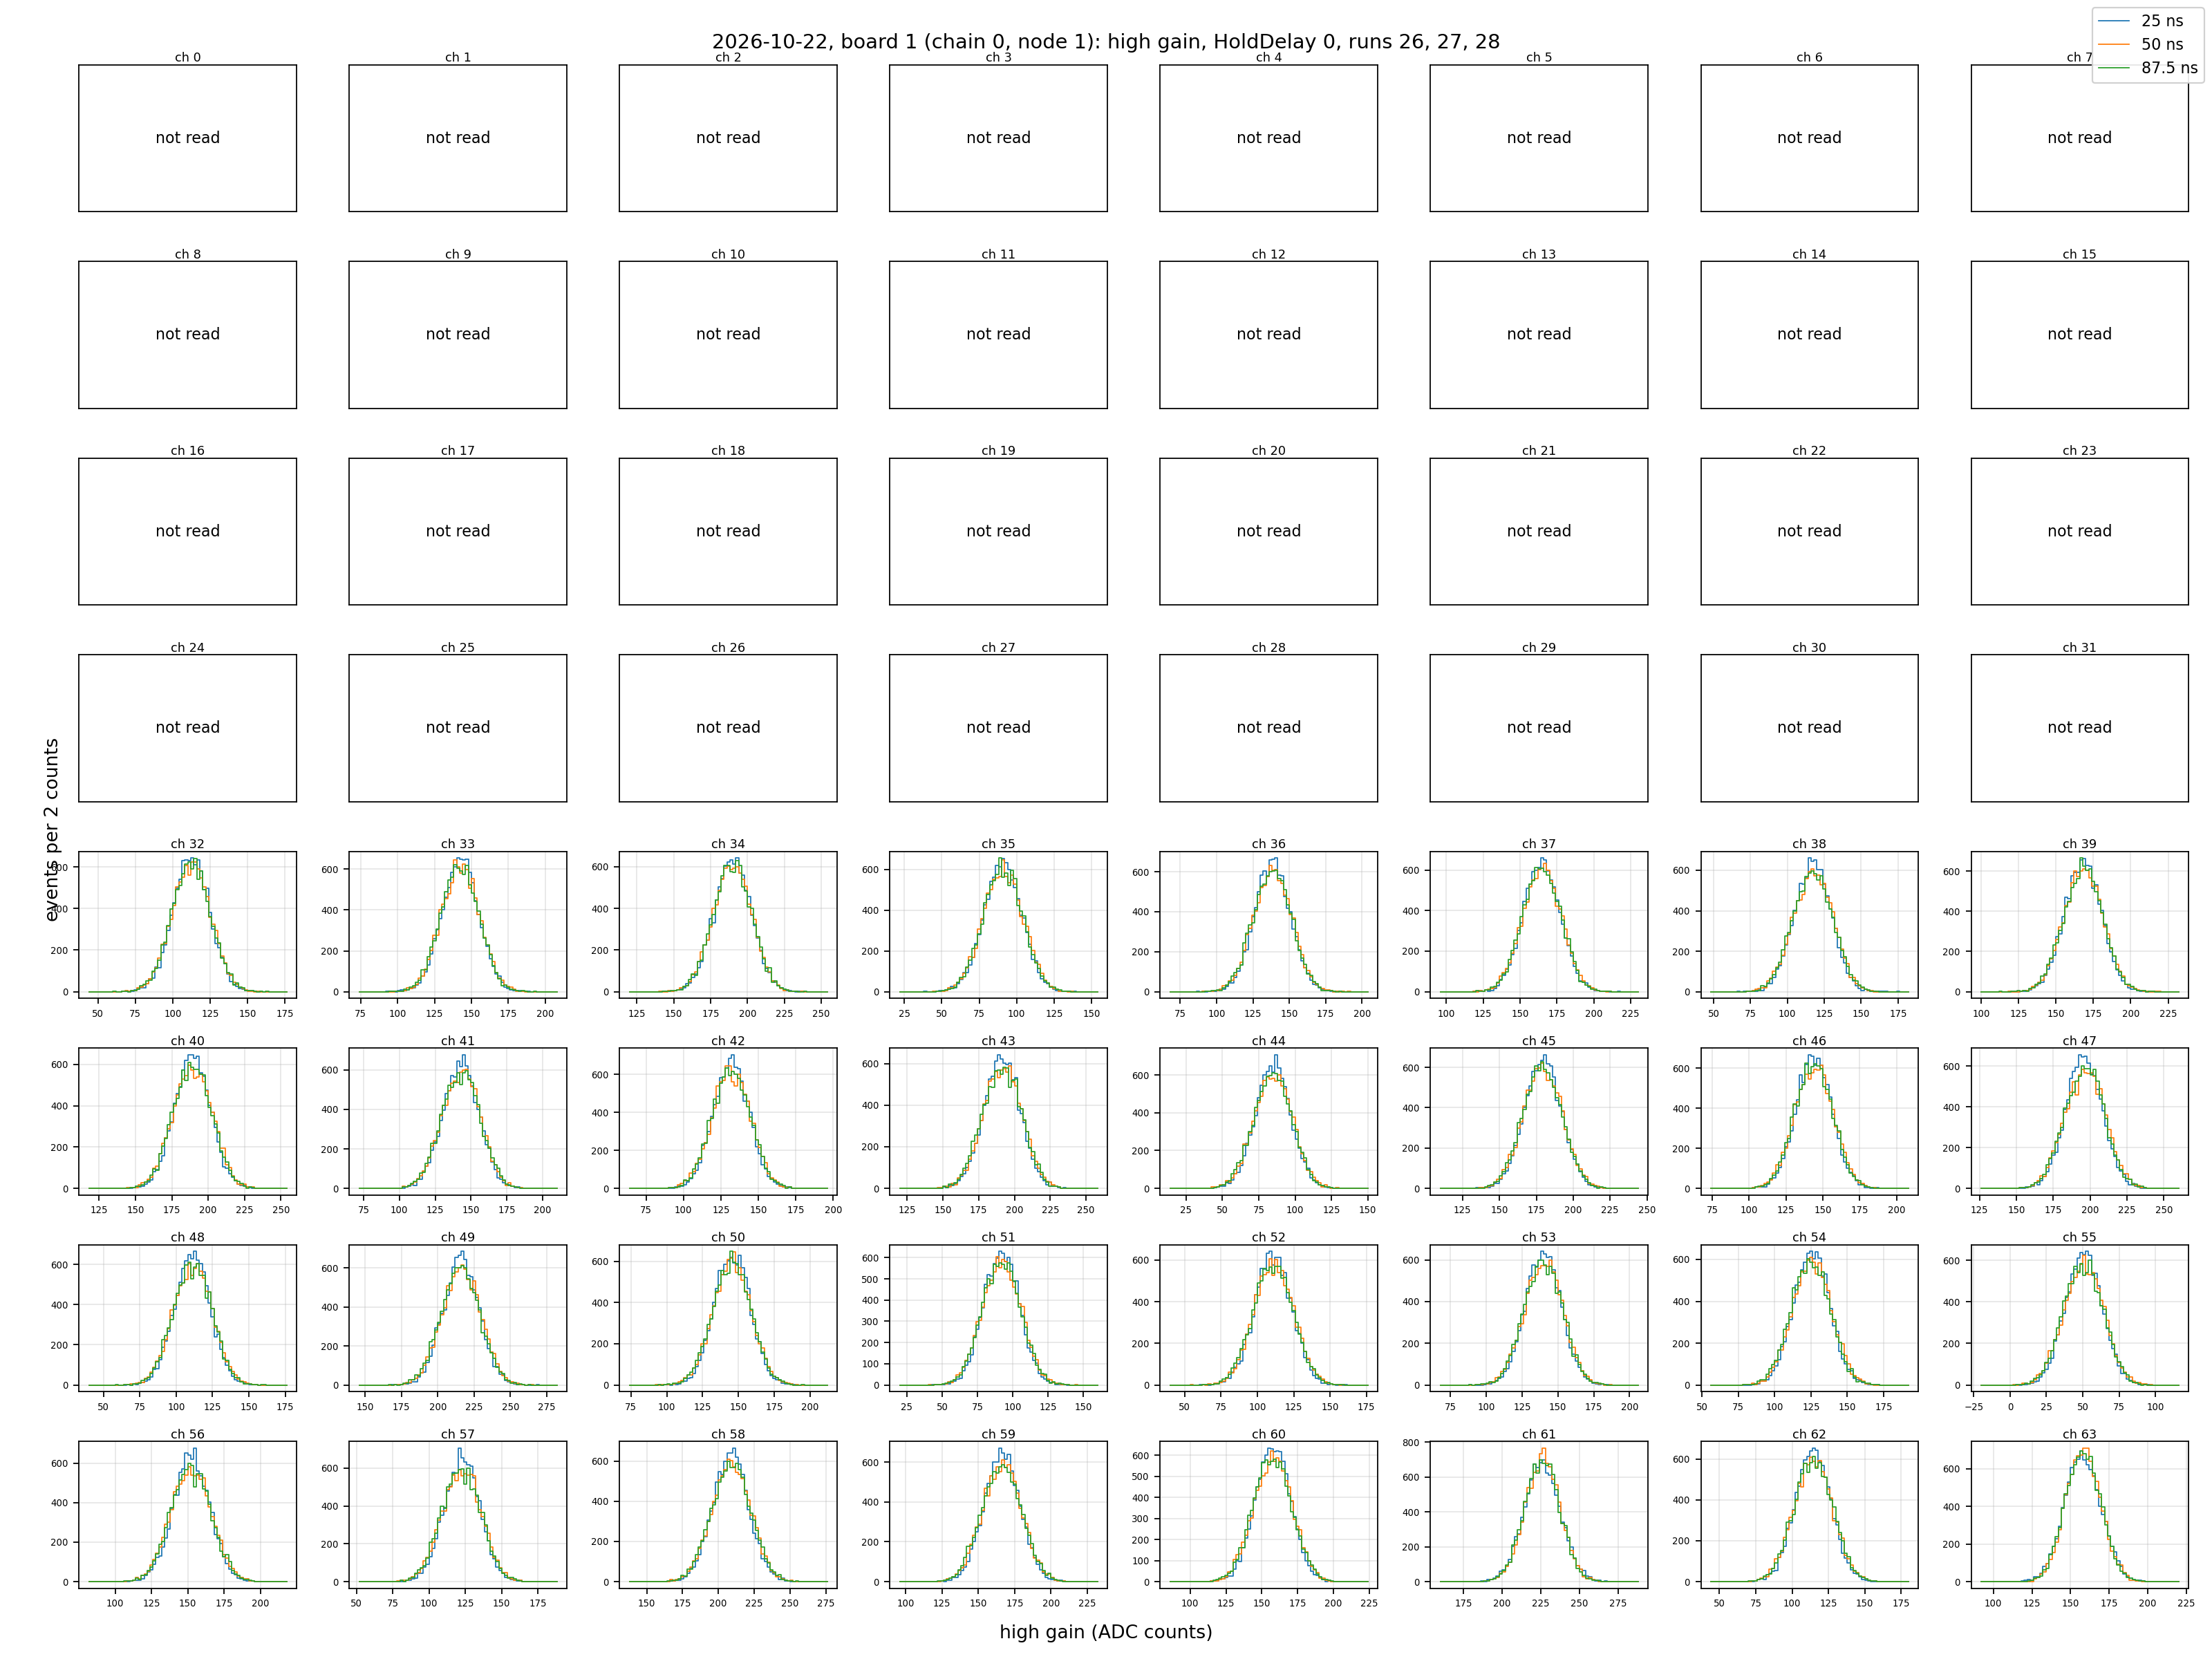
\includegraphics[width=\textwidth]{pedestal_spectra_board1.png}
\caption{Board 1: spectrum of the high gain of each channel in runs 26--28.}
\end{figure}
\begin{figure}[p]
\centering
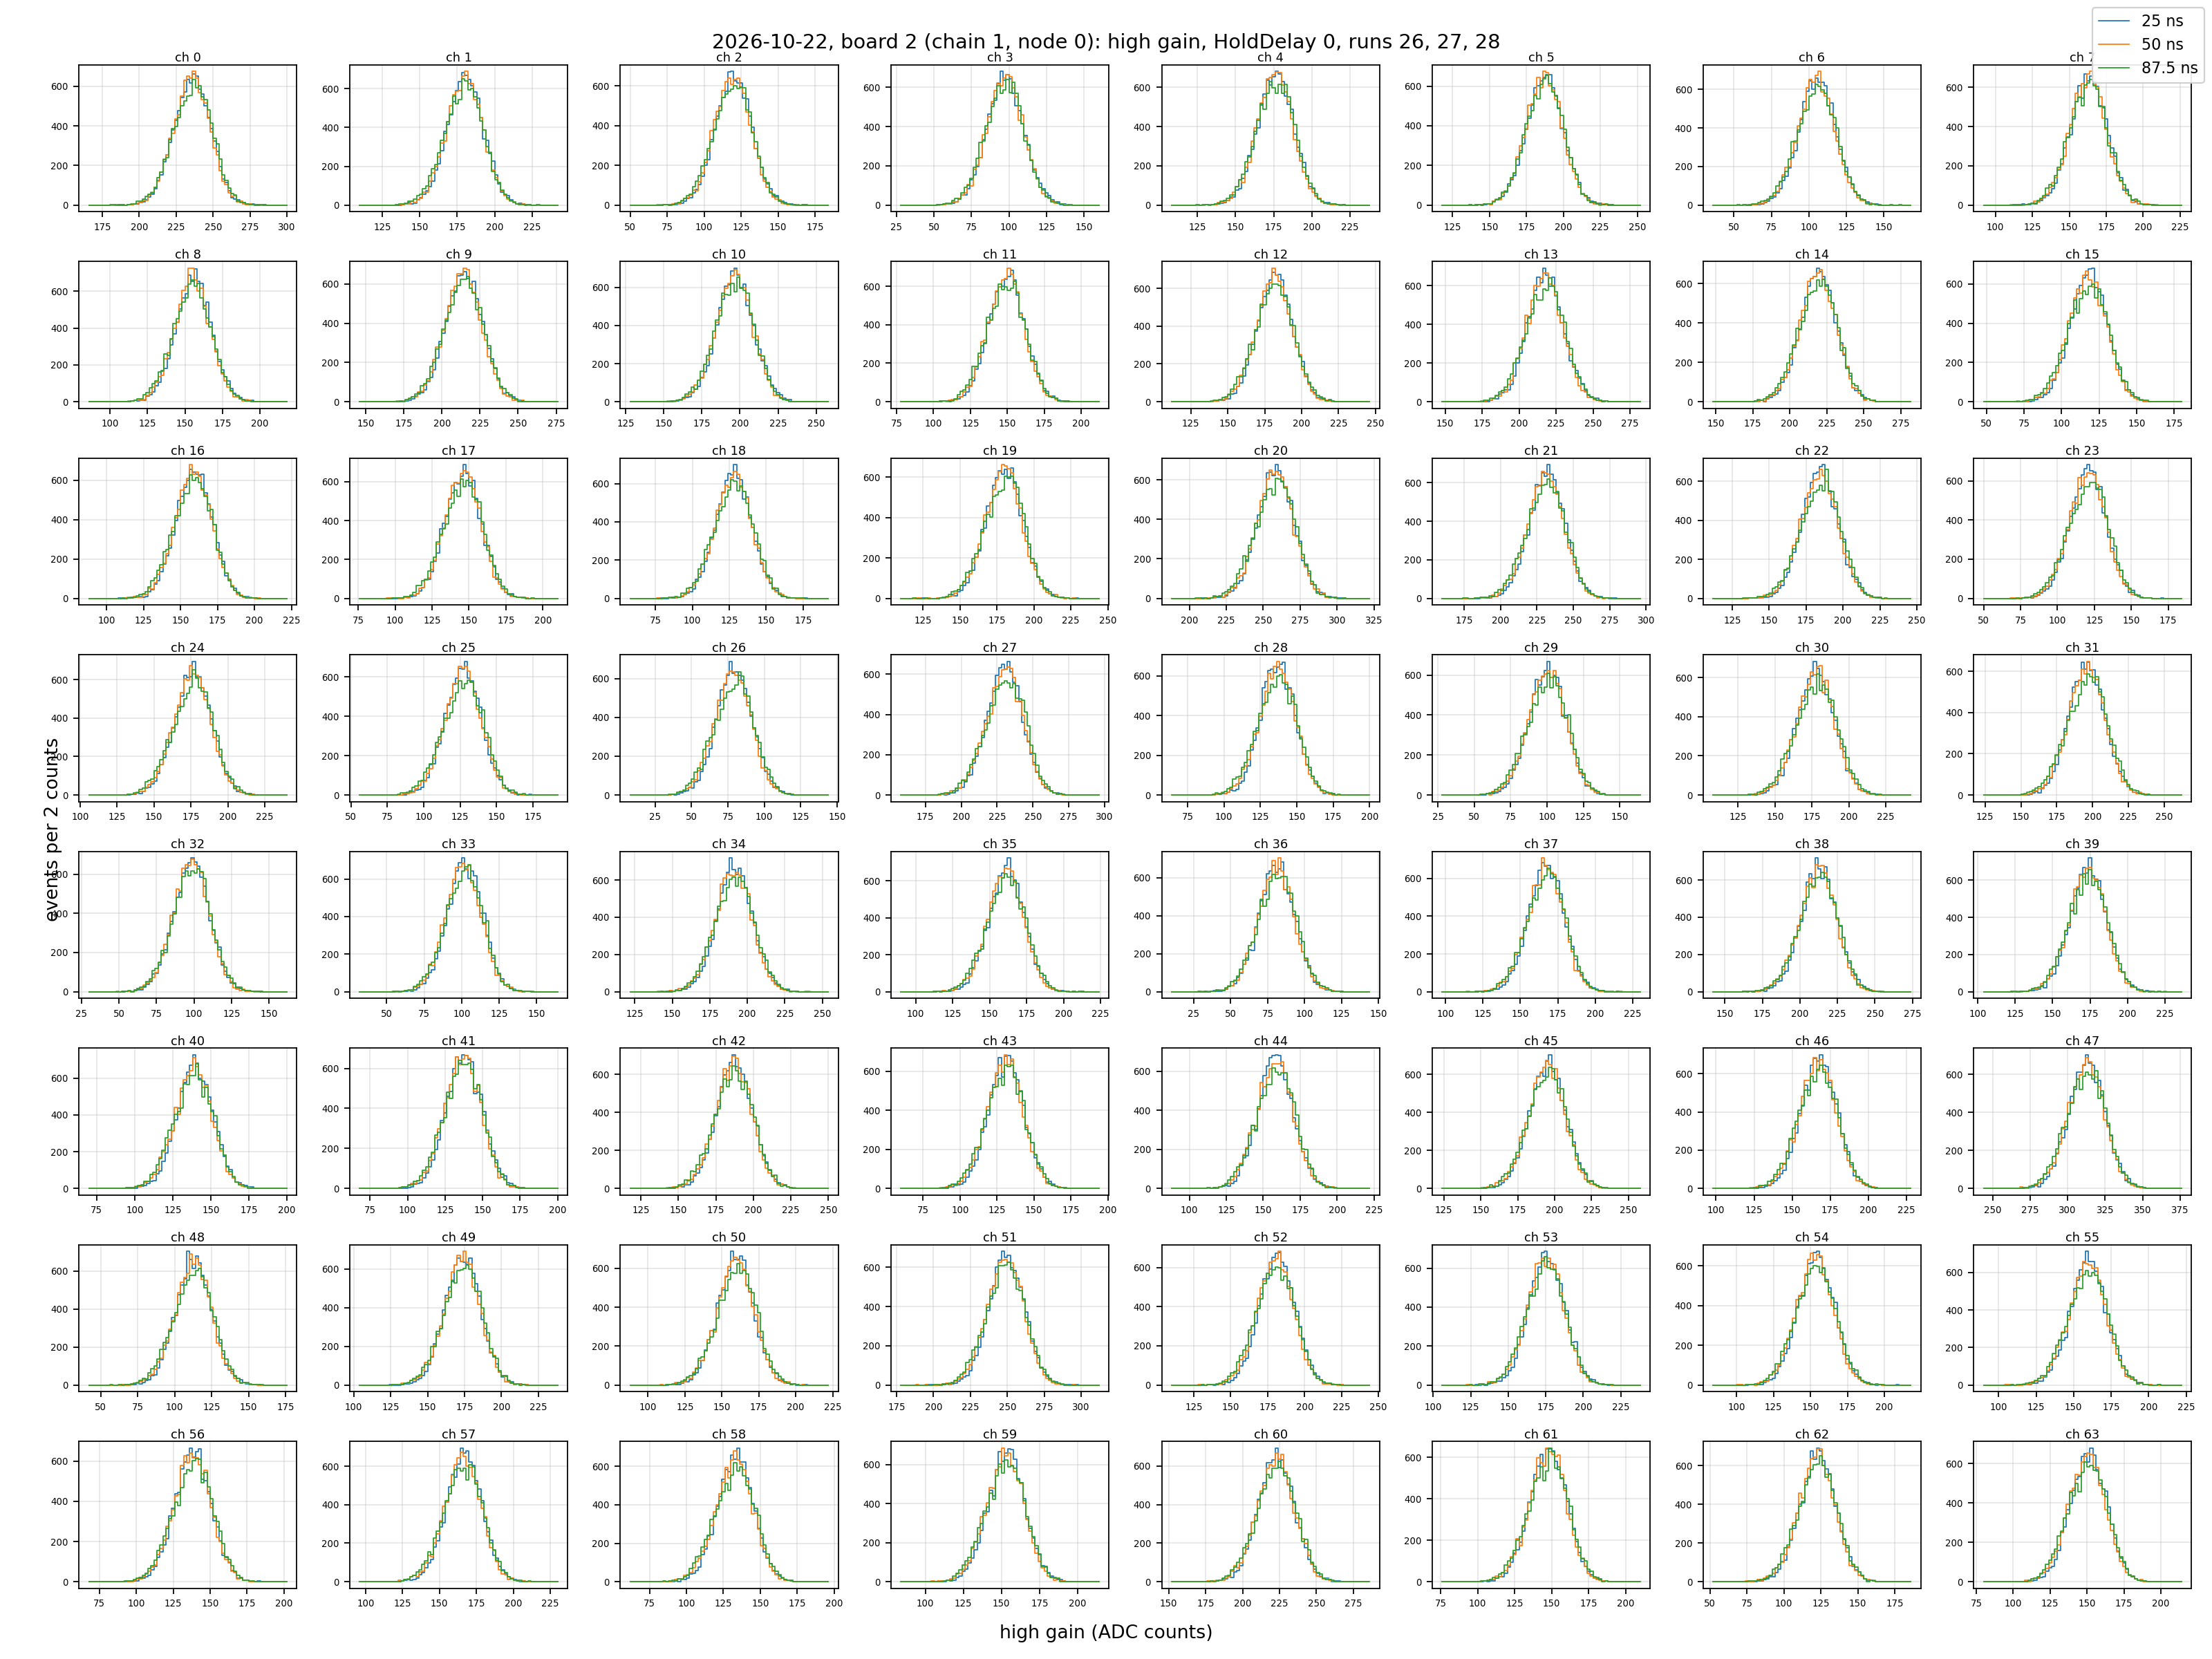
\includegraphics[width=\textwidth]{pedestal_spectra_board2.png}
\caption{Board 2: spectrum of the high gain of each channel in runs 26--28.}
\end{figure}
\begin{figure}[p]
\centering
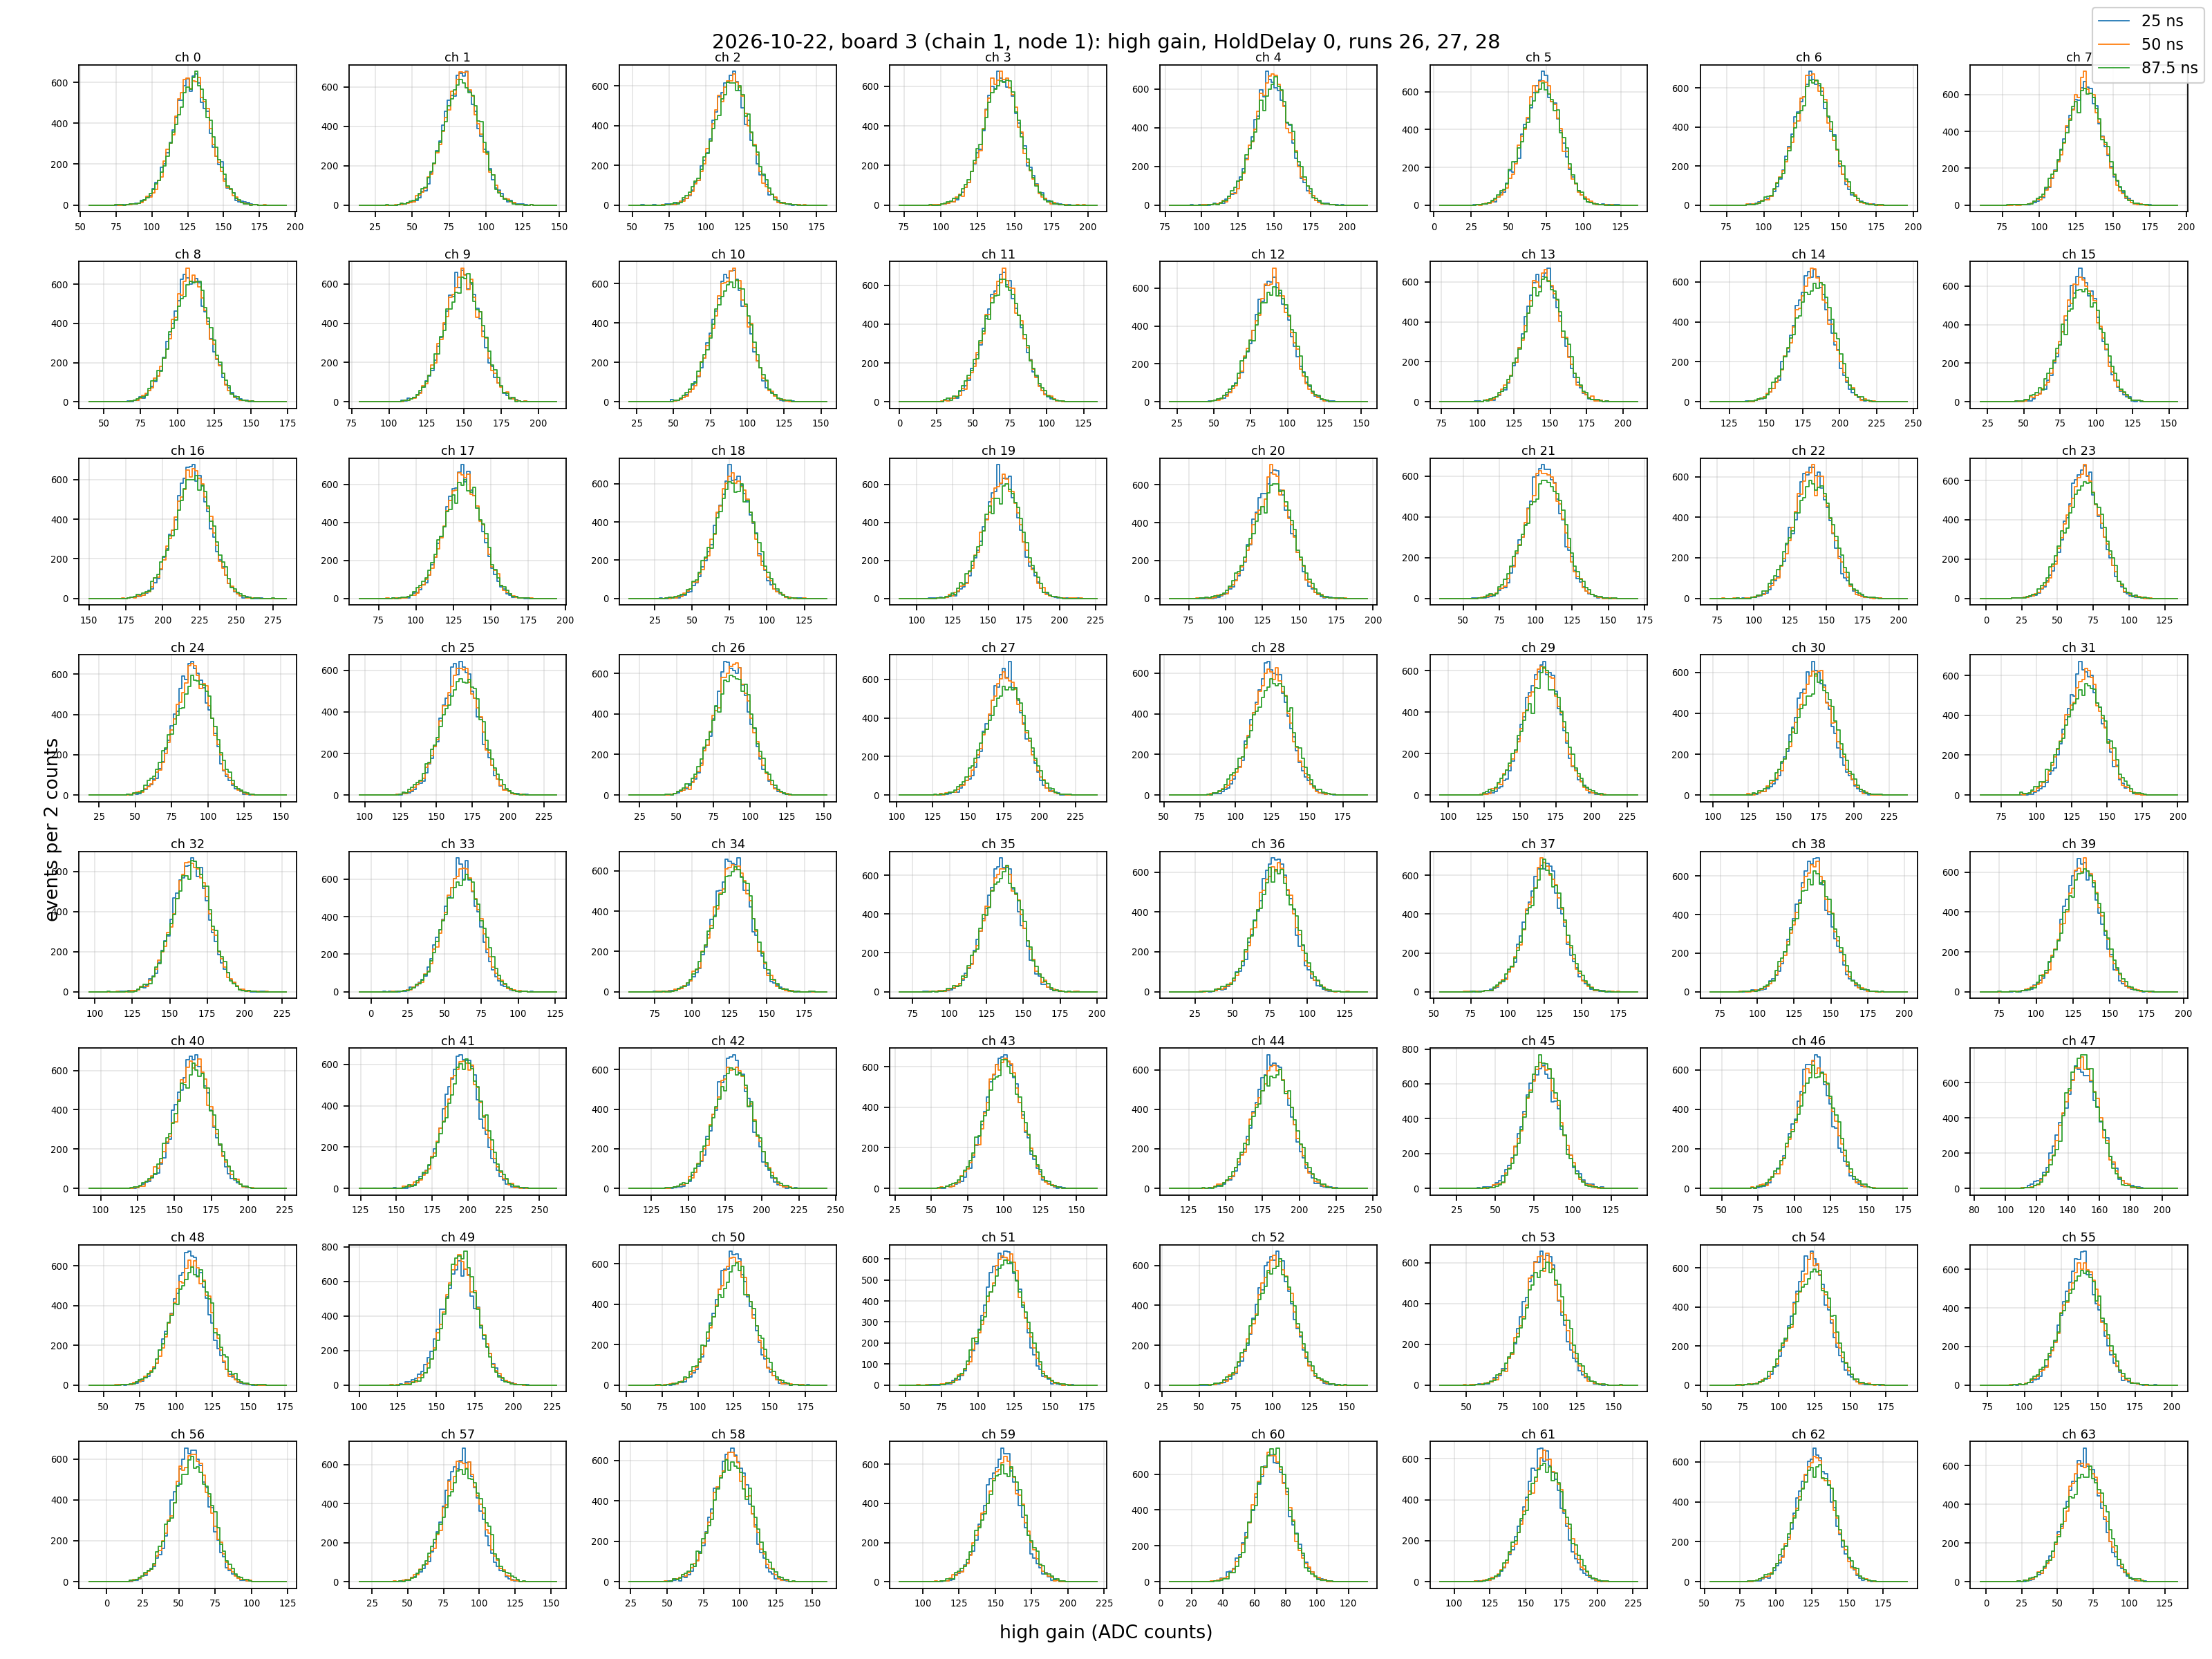
\includegraphics[width=\textwidth]{pedestal_spectra_board3.png}
\caption{Board 3: spectrum of the high gain of each channel in runs 26--28.}
\end{figure}
\begin{figure}[p]
\centering
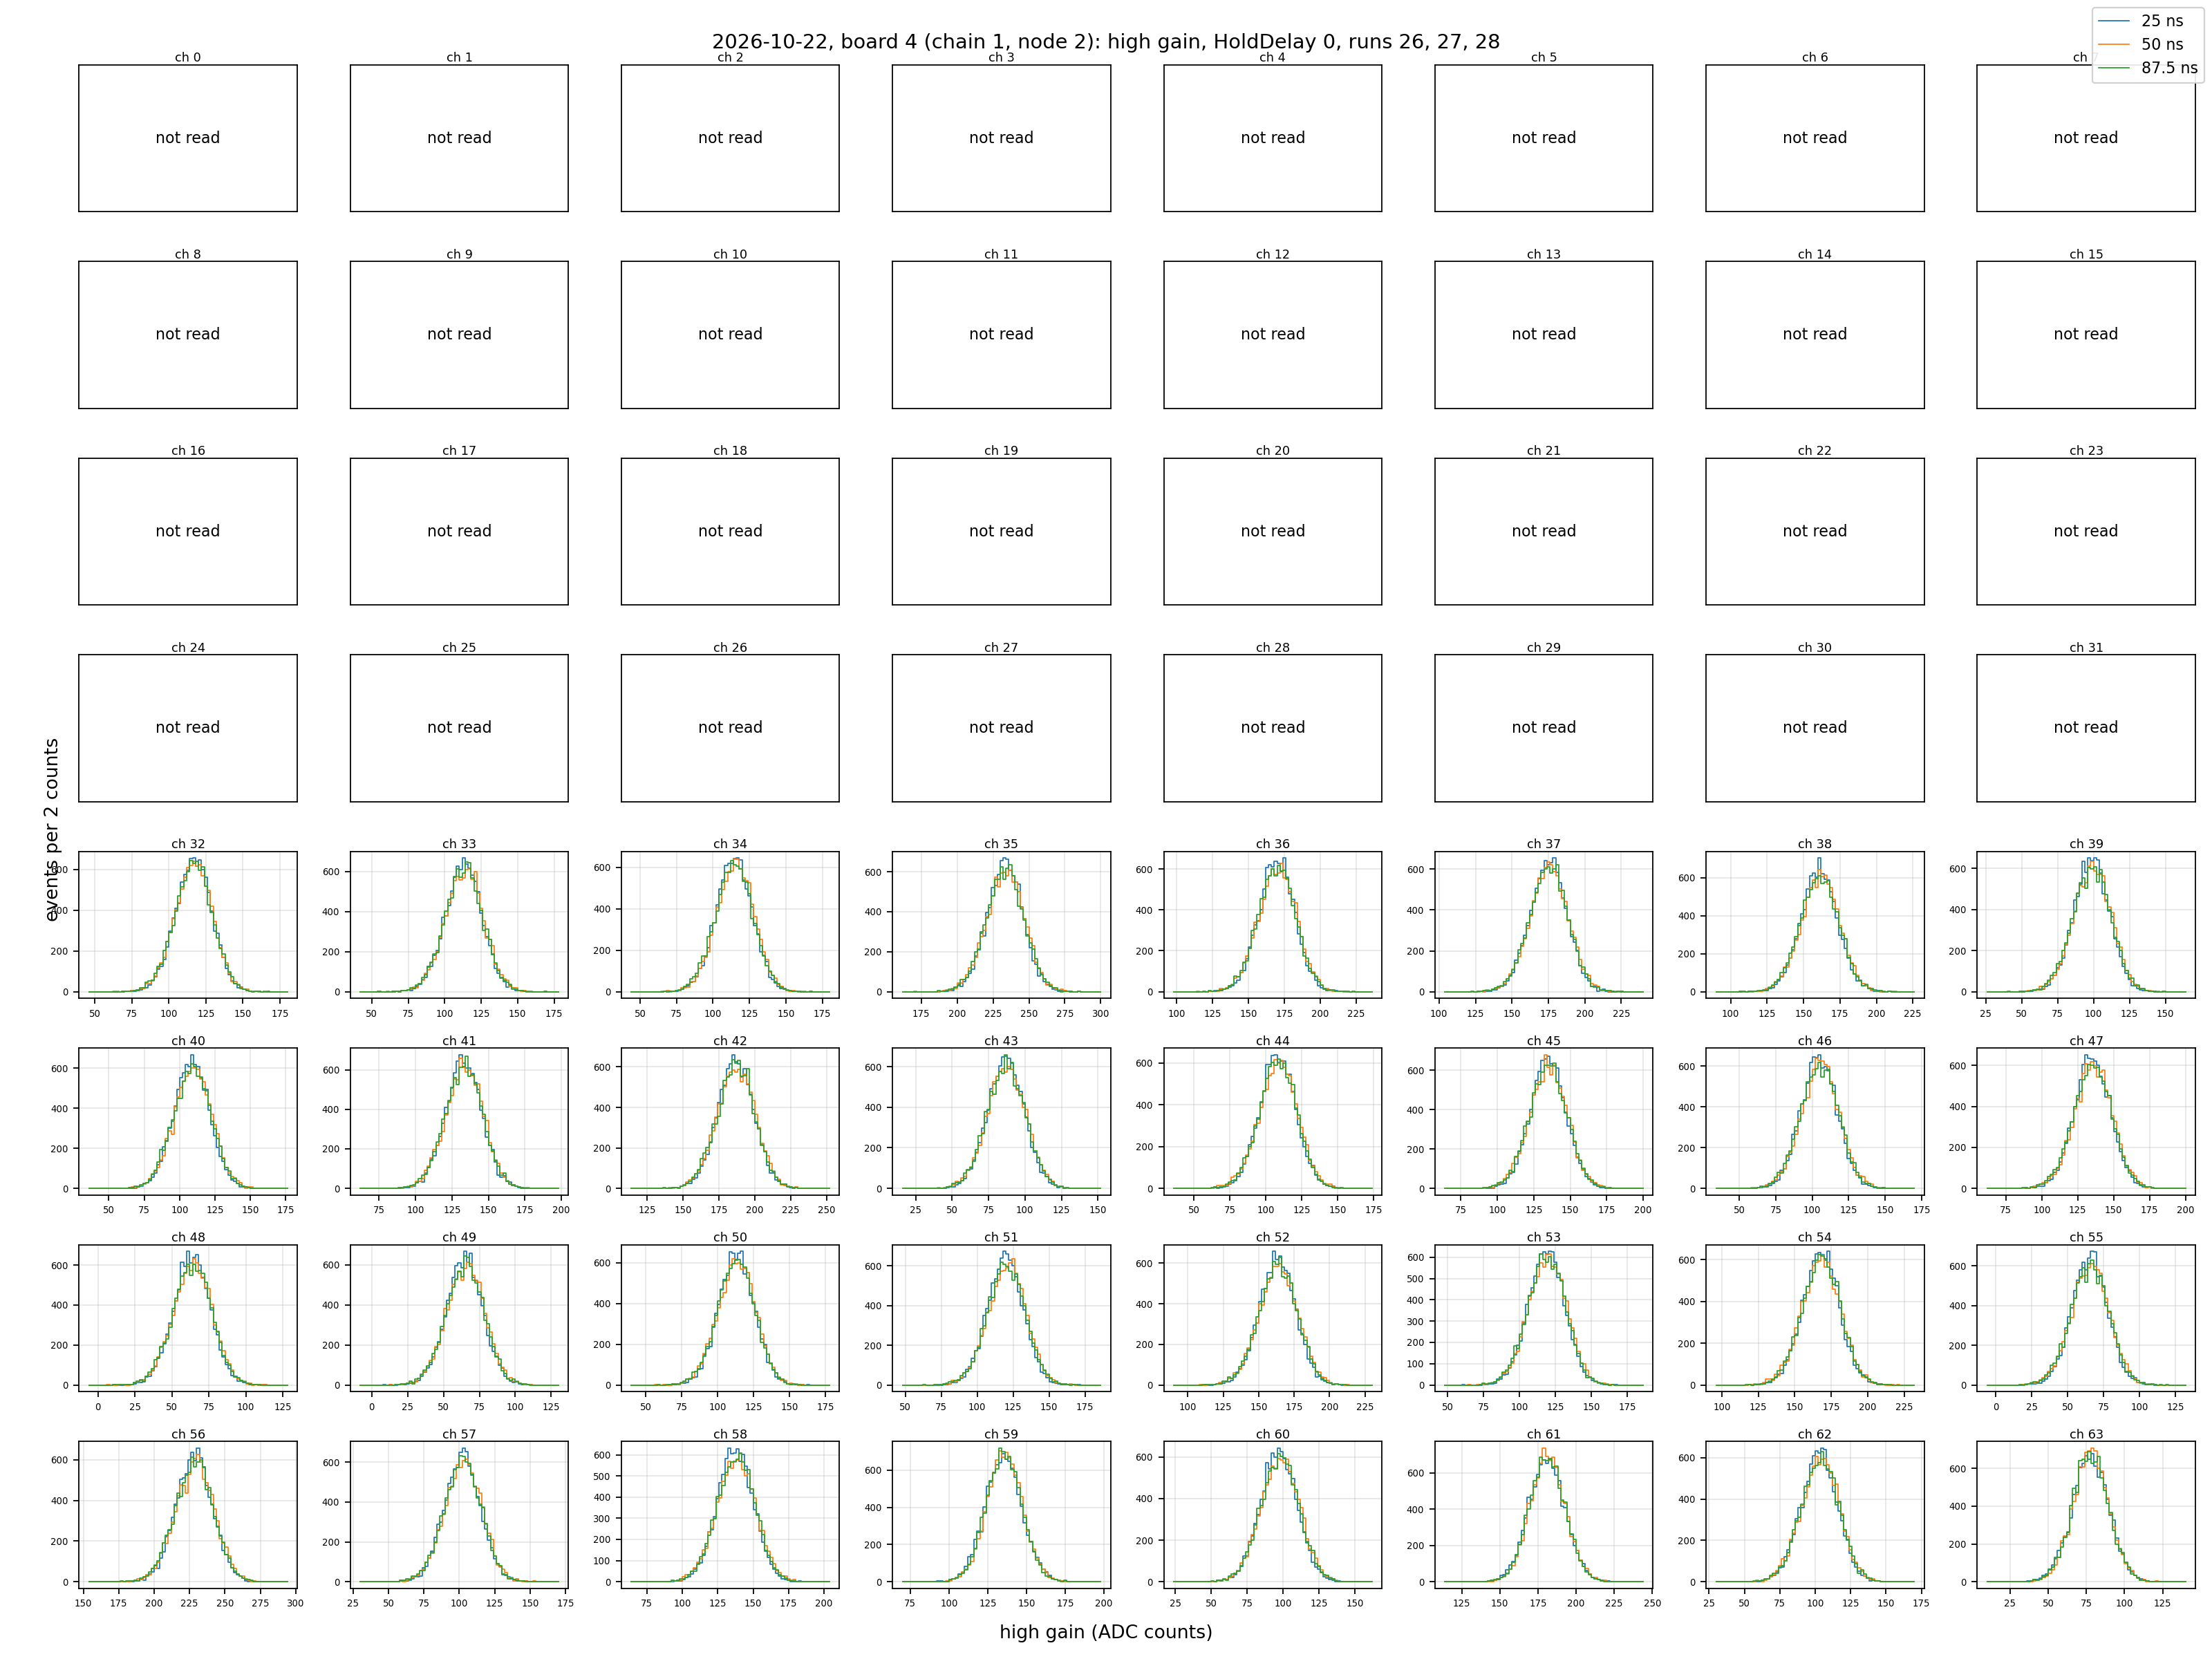
\includegraphics[width=\textwidth]{pedestal_spectra_board4.png}
\caption{Board 4: spectrum of the high gain of each channel in runs 26--28.}
\end{figure}

\end{document}
